Nástrojů jak dnes psát dokumenty máme celou řadu, některé jsou volně dostupné a jiné jsou zpoplatněny. Některé nástroje jsme si již představili (Word, LibreOffice), ale
nyní se zaměříme na takzvané značkovací jazyky. Značkovací jazyky nám umožnují psát text, který je poté možné zpracovat počítačem, který změní jeho formátování. Většina
značkovacích jazyků má jasně\linebreak rozlišitelné značky, nebo jinak také tagy, které upravují formátování při jejich strojovém překladu, díky tomu je původní text stále dobře čitelný.
\cite{markup} Výhodou je u nich, kromě jednoduché čitelnosti původního textu, volnost užití, není potřeba pro jejich úpravu žádný speciální software. Pokud je chceme převést do
konečné podoby, stačí nám k tomu volně dostupné nástroje, které jsou ve většině případů dostupné i online a není třeba je tedy instalovat na naše zařízení.

Mezi značkovací jazyky například patří i jazyky používané při\linebreak psaní webových stránek, jako je \gls{html} či \gls{xml}, ovšem tyto jazyky budeme spíše využívat pro zobrazování výstupu
jednodušších značkovacích jazyků. My se budeme hlavně zabývat těmito 3 jazyky: Markdown, reStructuredText a AsciiDoc. Tyto jazyky se používají pro psaní dokumentace v jednotlivých programech
(docutil, AsciiDoc) či slouží k vytváření uživatelských návodů (Markdown).
\clearpage

\section{Markdown}

Markdown je značkovací jazyk, který se typicky převádí do \gls{html}. Jedná se o jednoduše čitelný a zároveň jednoduchý jazyk na psaní strukturovaného textu. Hlavní myšlenkou Markdown je, že
text v něm psaný by měl být publikovatelný i bez jeho zpracování, inspirací tomuto přístupu jsou čistě textové emaily (emaily se dnes ve většině případů píšou v \gls{html}
z důvodu grafického obsahu). \cite{markdown}

Markdown se používá na některých verzovacích službách jako je například GitHub, ovšem v tomto případě se jedná o upravenou implementaci Markdown, která je rozšířena o další
tagy/značky. Podobnou úpravu Markdown má i konkurenční služba GitLab.

Takto vypadá menší ukázka Markdown syntaxe \ref{lst:markdown} a také výsledek, který je poté generován \ref{fig:markdown}.

\begin{listing}[ht]
    \inputminted[linenos,breaklines]{md}{example.md}
    \caption{Příklad Markdown syntaxe}
    \label{lst:markdown}
\end{listing}

\clearpage

\section{reStructuredText}

Formát reStructuredText pro psaní dokumentů v prostém textu, který je snadný na čtení, kde je hned zřejmé, jak bude vygenerovaný text vypadat.
Tento formát je jednoduchý na použití hlavně pro psaní programátorské dokumentace, menších webů a samostatných dokumentů.
Hlavním cílem reStructuredText je definovat a uplatnit jednoduchý značkovací jazyk pro použítí v Python, kde se používá k dokumentaci jednotlivých částí programu,
a dalších dokumentačních nástrojích, který je jednoduše čitelný a jednoduše použitelný. \cite{reStruDoc}

\uv{Docutil je open-source program pro zpracovaní dokumentace v textové podobě do, pro uživatele, přívětivého formátu, jako je například \gls{html}, \LaTeX~či \gls{xml}.} \cite{docutil}
Docutil používá jako vstupní formát již zmíněný reStructuredText. Pro převod do formátu \gls{pdf} lze poté použít utilitu Pandoc \cite{pandocSW}, která umí převěst různé značkovací jazyky
na ostatní formáty jako například náš rst (reStructuredText formát) a to nejenom do \gls{pdf}, ale také do formátů jako je Markdown, \gls{html} a dalších.
Pandoc lze také přímo využít v Pythonu, díky modulu pypandoc \cite{pypandocSW}.

Stejně jako u Markdown, zde máme ukázku syntaxe \ref{lst:rst} i výsledného dokumentu \ref{fig:rstOutput}.

\begin{listing}[ht]
    \inputminted[linenos,breaklines]{rst}{example-rst.rst}
    \inputminted[linenos,breaklines]{rst}{module.rst}
    \caption{Příklad reStructuredText syntaxe}
    \label{lst:rst}
\end{listing}

\clearpage

\section{AsciiDoc}

AsciiDoc je další formát pro psaní dokumentu, jedná se stejně jako reStructuredText, o modul pro jazyk Python. Tento modul je možné použít pro psaní nejenom poznámek,
ale je možné jej exportovat i do formátů jako jsou .epub (formát pro elektronické čtečky knih), či \gls{pdf}. \cite{asciiDoc} Syntaxe jazyku je podobná reStructuredText.

Projekt byl původně psán pro jazyk Python, ovšem posléze byla syntaxe adoptována jako balíček pro jazyk Ruby a také přejmenován na AsciiDoctor \cite{asciiDoctorSW}. AsciiDoctor lze posléze
použít i přímo v kódu, a to konkrétně v jazyce Ruby, zde je menší ukázka nejenom formátu asciiDoc, ale i jeho použití v kódu.

Ukázka syntaxe \ref{lst:asciiDoc} a výsledného dokumentu i pro AsciiDoc je vidět na obrázku \ref{fig:asciiOutput}.

\begin{listing}[ht]
    \inputminted[linenos,breaklines]{text}{example-ascii.adoc}
    \inputminted[linenos,breaklines]{text}{module.adoc}
    \begin{minted}[linenos,breaklines]{ruby}
        # example.rb
        require 'asciidoctor'

        Asciidoctor.convert_file 'example.adoc', to_file: true, safe: :safe
    \end{minted}
    \caption{Příklad AsciiDoc syntaxe a ukázka použití AsciiDoctor}
    \label{lst:asciiDoc}
\end{listing}

\clearpage

\section{Porovnání}

Po představení těchto 3 jazyků je nyní na čase porovnat je, zhodnotit jejich použitelnost pro modulární dokumenty a vybrat si, který použijeme v rámci naší aplikace.
V rámci porovnání musíme dát hlavně důraz na podporu modularity v rámci jazyka, tedy jestli je už v samostatném značkovacím jazyku podpořeno vkládání dalších
souborů s textem, tedy modulů. Dále se také zaměříme na jednoduchost generování různých formátů, některé jazyky jsou podpořeny v Pandocu a pokud jsou, do jakých
formátů je lze převést.

Prvně začněme s jazykem Markdown, jeho představení už máme za sebou a nyní se podívejme na možnost jeho využití při vytváření modulárních dokumentů. Bohužel
Markdown nepodporuje přímé vkládání dalších souborů, tento nedostatek jej činí, oproti ostatním 2 jazykům, nepoužitelným pro modulární dokumenty. Je zde sice možná úprava
kódu, který by text obohatil o moduly před výsledním zpracováním, ale tato úprava by byla náročná na provedí v takovém rozsahu, abychom mohli zaručit její bezchybnost.

Dalším na řadě je reStructuredText, tento jazyk má možnost vkládat v rámci jednoho souboru i další soubory, které obashují další kód, díky této vlastnosti
lze u něho použít modulární přístup k vytváření dokumentů bez žádného předzpracování textu. Tento jazyk je podporován v rámci Pandocu \cite{pandocSW} a je možné
jej převest nejenom do formátu \gls{pdf}, ale i spousty další, jmenovitě například: Markdown, EPUB (formát pro čtečky knih) či již zmíněné \gls{pdf}.

AsciiDoc je poslední jazyk na porovnání, stejně jako reStructuredText, nám i AsciiDoc nabízí možnost připojení dalších souborů, které budou převedeny na výsledný dokument.
Protože je ovšem již podporován pouze v jazyce Ruby, budeme potřebovat na jeho převod do výsledných formátů instalovat jednotlivé moduly pro tento jazyk. Bohužel nelze
vyzužít Pandoc, neboť tuto verzi AsciiDocu již nepodporuje. Použijeme tedy nástroj AsciiDoctor \cite{asciiDoctorSW}, tento nástroj nám výsledný dokument umí převést do
formátu \gls{html}, pro převod do jiných formátů jako například \gls{pdf} je nutné mít kromě AsciiDoctor nainstalováno i jeho rozšíření asciidoctor-pdf \cite{asciidoctorpdfSW}.
Toto trochu znevýhoďnuje AsciiDoc oproti reStructuredText, který má výhodu v možnosti použití jednoho nástroje na převod do vícero formátů.

Na závěr tohoto porovnání je třeba uvést jaký jazyk budeme v naší aplikaci používat. Tímto jazykem bude reStructuredText a to z několika důvodů:
\begin{enumerate}
    \item Prvním důvodem je jeho snadný převod do ostatních formátů díky nástroji Pandoc \cite{pandocSW} a jeho modulu pypandoc \cite{pypandocSW}, který nám umožní používat Pandoc v přímo v aplikaci.
    \item Druhým důvodem je autorova předešlá zkušenost v jazyce Python a také zkušenosti s nástojem Pandoc a modulem pypandoc.
\end{enumerate}

\begin{figure}[h]
    \centering
    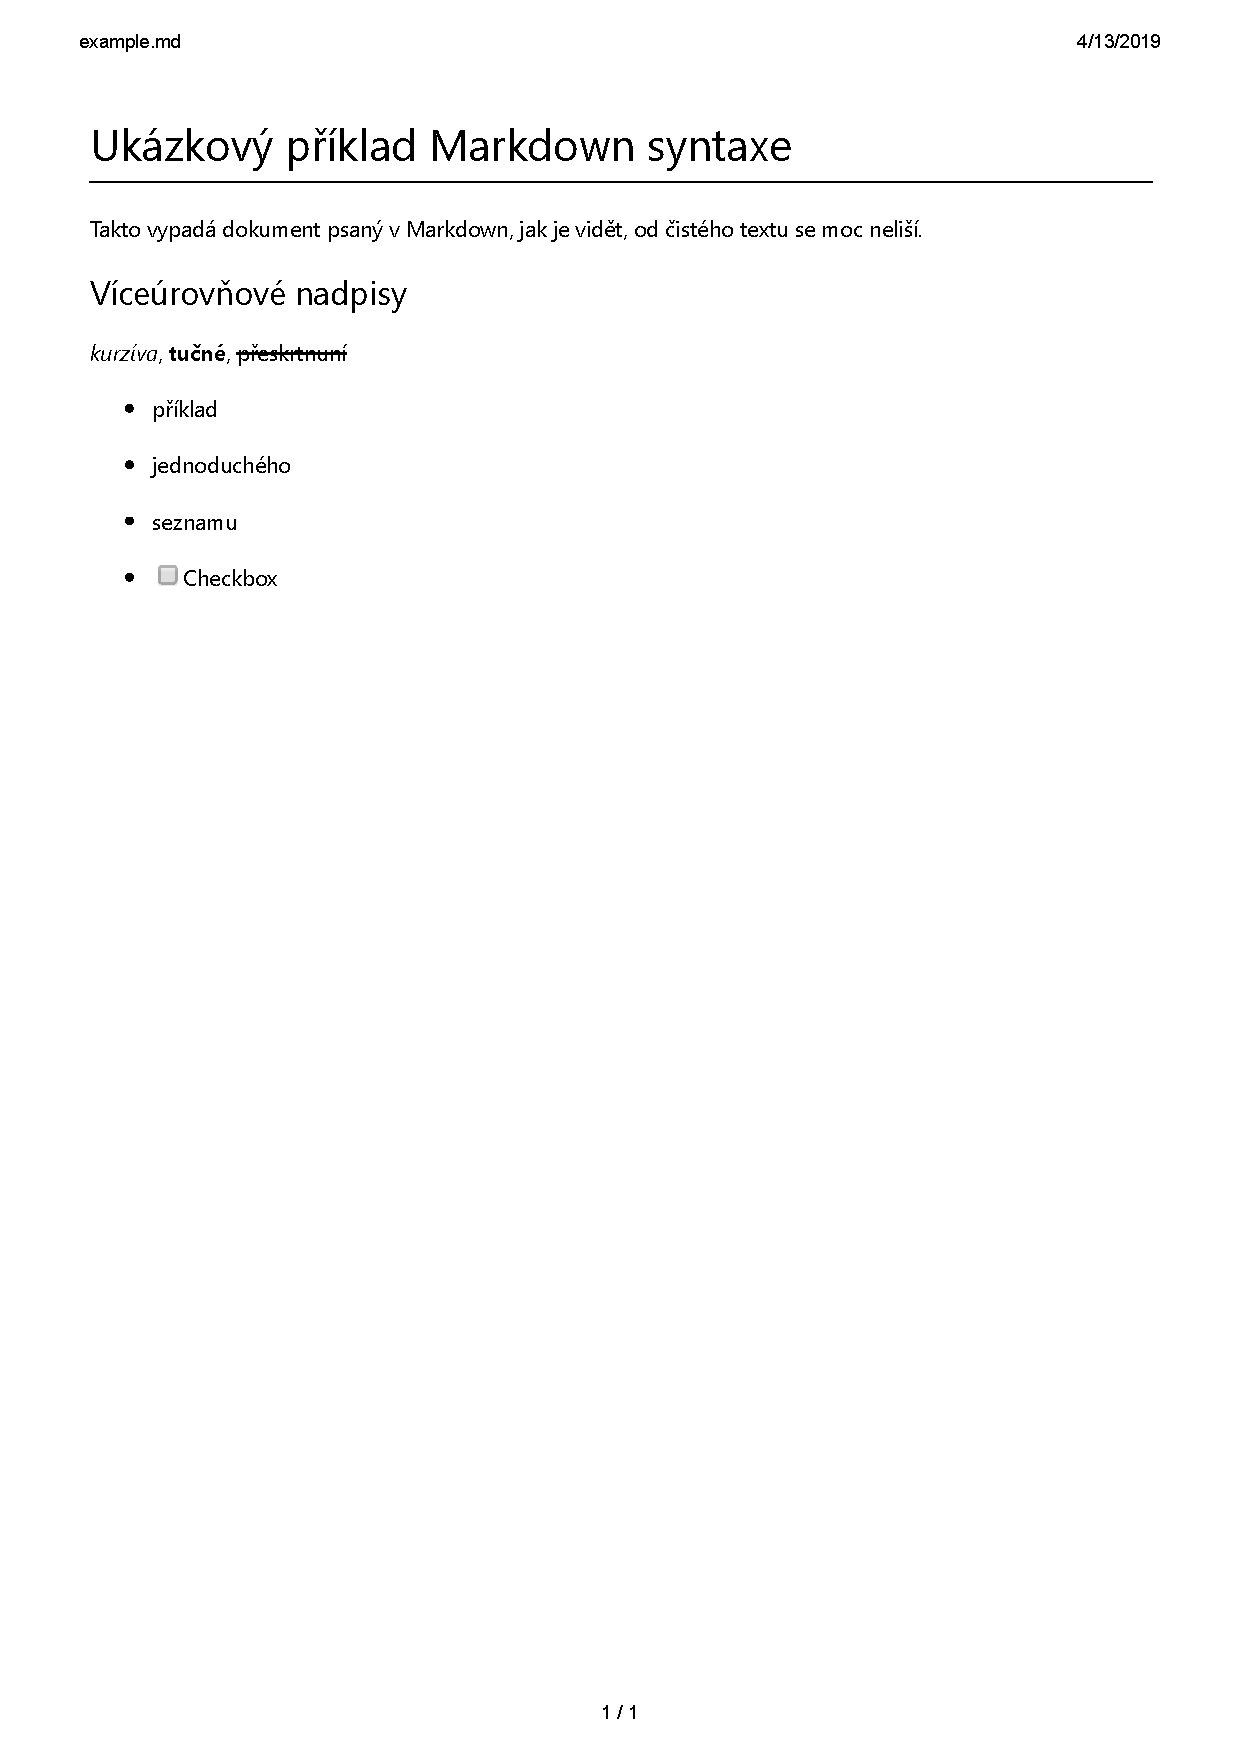
\includegraphics[width=\textwidth]{example.pdf}
    \caption{Výstup Markdown}
    \label{fig:markdown}
\end{figure}

\begin{figure}[h]
    \centering
    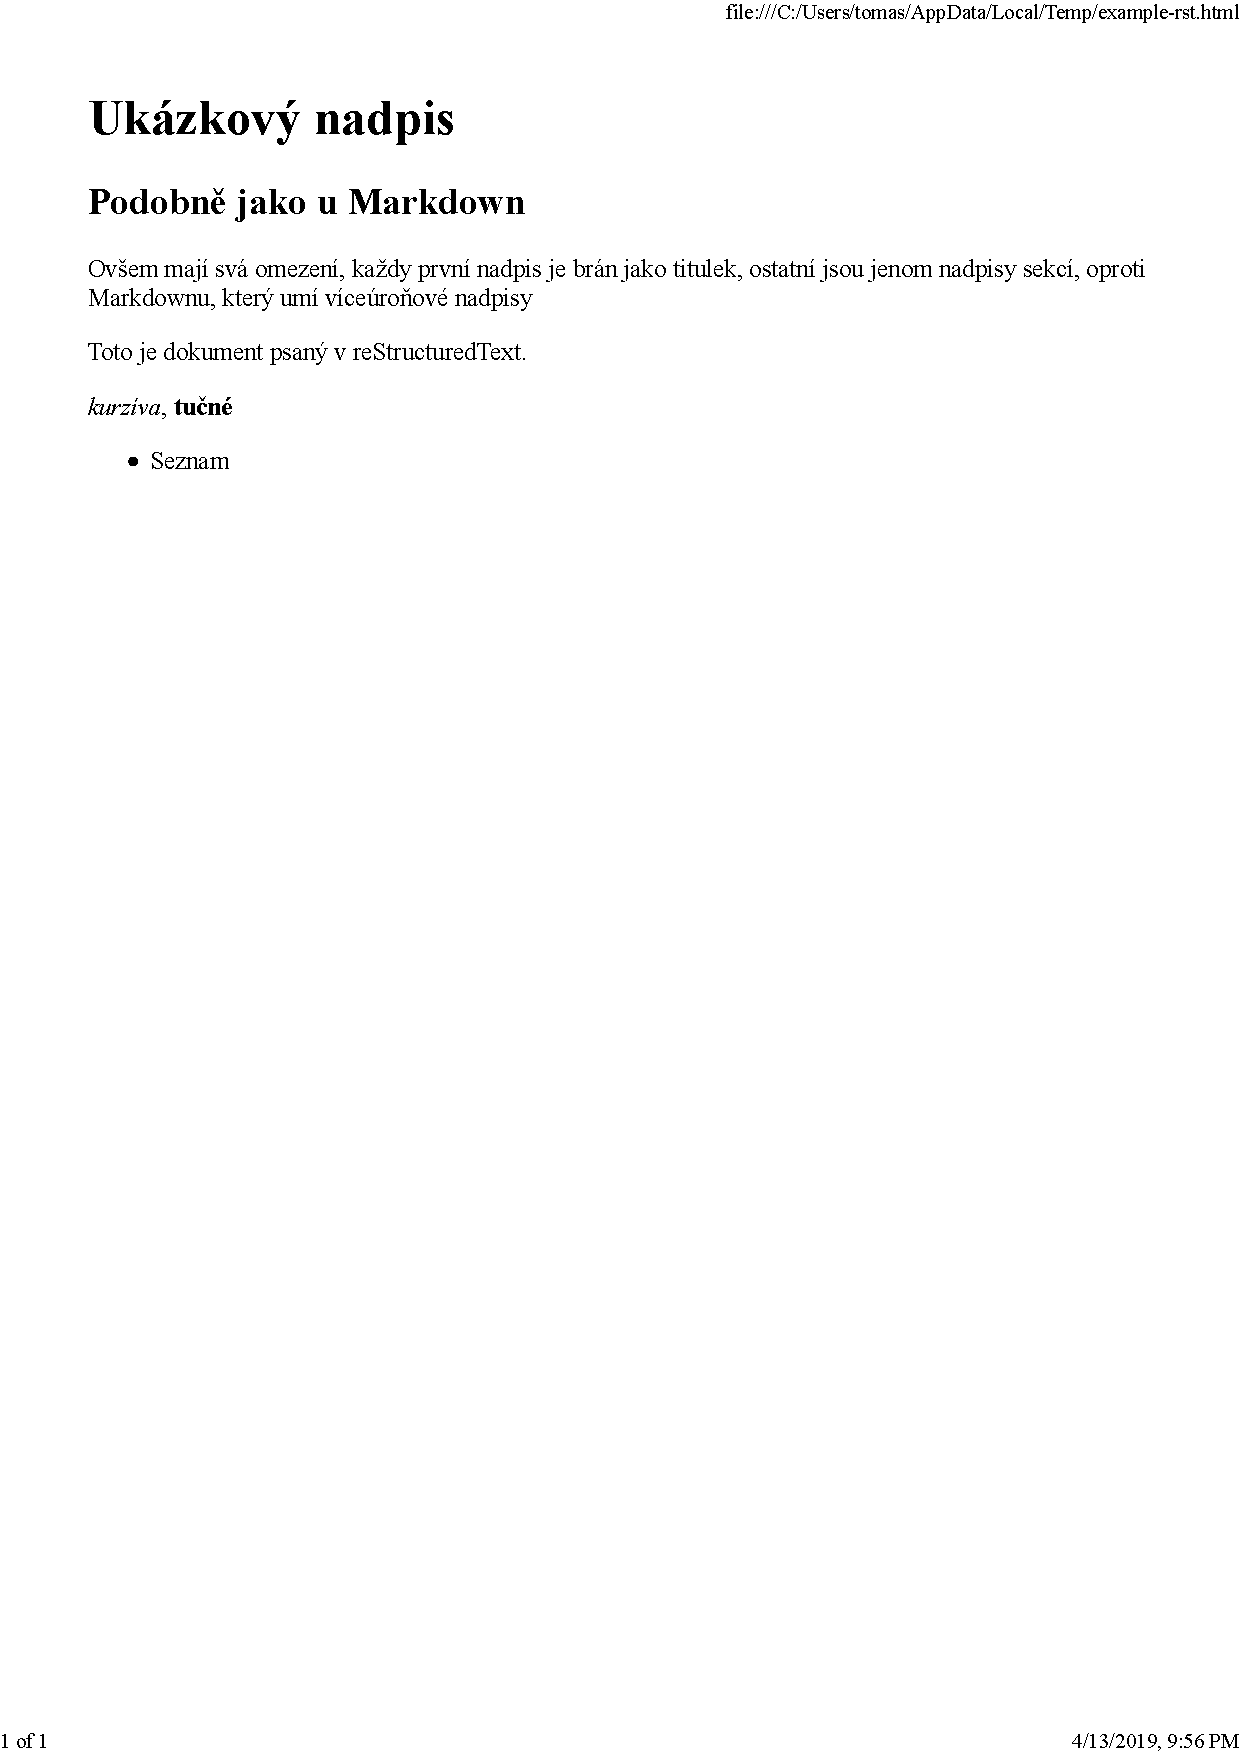
\includegraphics[width=\textwidth]{example-rst.pdf}
    \caption{Výstup reStructuredText}
    \label{fig:rstOutput}
\end{figure}

\begin{figure}[h]
    \centering
    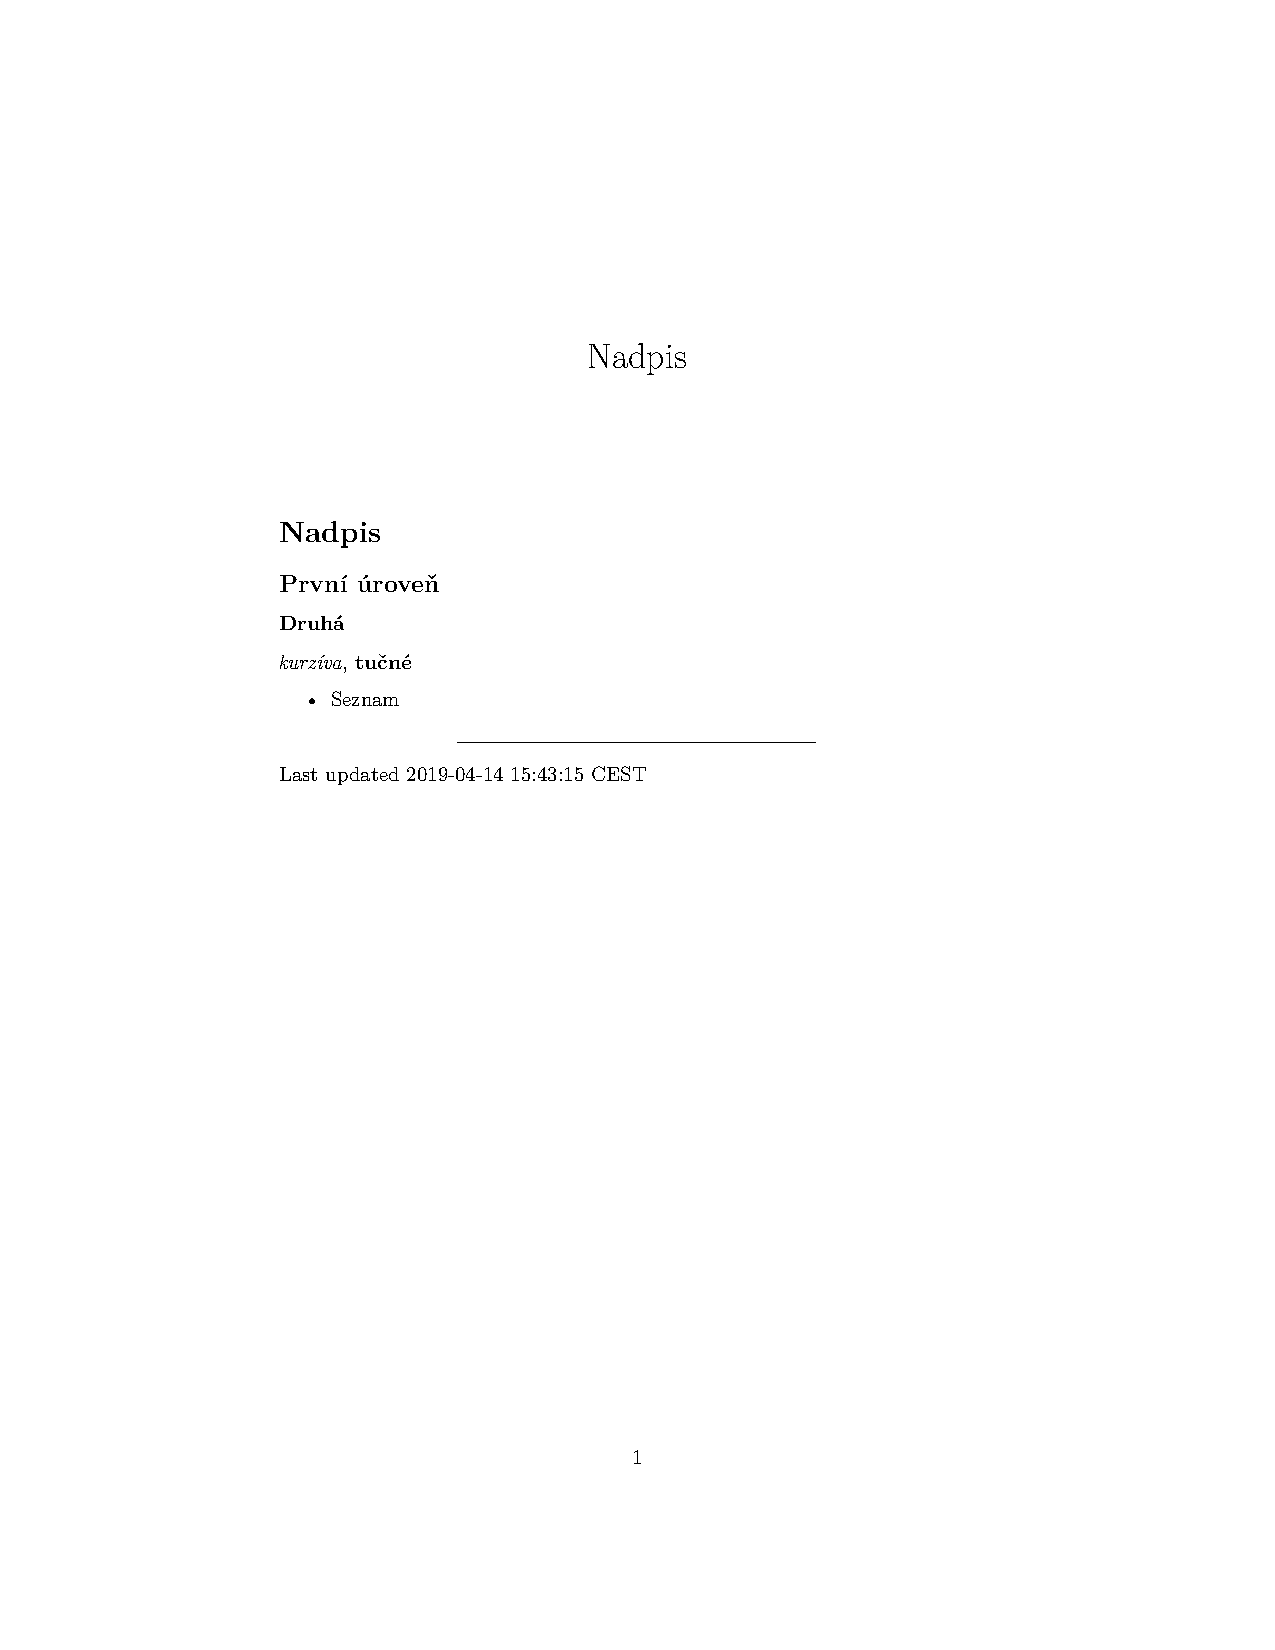
\includegraphics[width=\textwidth]{example-ascii.pdf}
    \caption{Výstup AsciiDoc}
    \label{fig:asciiOutput}
\end{figure}
